\documentclass[uplatex,a4paper,12pt]{jsarticle}

%% フォント
%\usepackage{newtxtext,newtxmath}
%% 図、文字色
\usepackage[dvipdfmx]{graphicx,xcolor}
%% ハイパーリンク
\usepackage[dvipdfmx]{hyperref}
%% しおりの日本語
\usepackage{pxjahyper}
%% しおりに節番号を含める、リンクの枠を出力しない
\hypersetup{
  bookmarksnumbered=true,
  hidelinks=true,
  colorlinks=false,
}
%% 特殊記号
\usepackage{textcomp}
%% URL
\usepackage{url}
%% 表
%\usepackage{multirow}
%% 参照漏れチェック（デバッグ用）
%\usepackage{refcheck}

% キャプションとページ番号をゴシック体に
\renewcommand{\kanjifamilydefault}{\gtdefault}
\usepackage{caption}
\usepackage{fancyhdr,lastpage}
\fancypagestyle{foot}
{
  \lhead{}
  \chead{}
  \rhead{}
  \cfoot{{\sf \thepage{}/{}\pageref{LastPage}}}
  \renewcommand{\headrulewidth}{0.0pt}
}

\usepackage[top=30truemm,bottom=30truemm,left=30truemm,right=30truemm]{geometry}
\usepackage{here}
\usepackage{fancyhdr}
\usepackage{lastpage}
\fancypagestyle{mypagestyle}{%
\lhead{}%ヘッダ左を空に
\rhead{}%ヘッダ右を空に
\cfoot{\thepage/\pageref{LastPage}}%フッタ中央に"今のページ数/総ページ数"を設定
\renewcommand{\headrulewidth}{0.0pt}%ヘッダの線を消す
}
\pagestyle{mypagestyle}
\begin{document}

% http://www.latex-cmd.com/style/style.html
% \gt % ゴシック体
% \sf % サンセリフ体
\gtfamily\sffamily

\makeatletter
\renewcommand{\section}{\@startsection{section}{1}{\z@}{1.5\Cvs \@plus.5\Cvs \@minus.2\Cvs}{.5\Cvs \@plus.3\Cvs}{\reset@font\bfseries\gtfamily\sffamily}}
\renewcommand{\subsection}{\@startsection{subsection}{1}{\z@}{1.5\Cvs \@plus.5\Cvs \@minus.2\Cvs}{.5\Cvs \@plus.3\Cvs}{\reset@font\bfseries\gtfamily\sffamily}}
\renewcommand{\subsubsection}{\@startsection{subsubsection}{1}{\z@}{1.5\Cvs \@plus.5\Cvs \@minus.2\Cvs}{.5\Cvs \@plus.3\Cvs}{\reset@font\bfseries\gtfamily\sffamily}}
\newenvironment{sftabular}[1]{\sffamily \begin{tabular}{#1}}{\end{tabular}}
\makeatother
\captionsetup[figure]{font=sf}
\captionsetup[table]{font=sf}
\captionsetup[lstlisting]{font=sf}
\pagestyle{foot}

\pagenumbering{arabic}
\setcounter{page}{1}

% タイトルとサブタイトル（ad-hoc）
%% maketitleでタイトルを入れたければ、プリアンブルを調整して同じ様に表示されるようにしてください。
\begin{center}
\fontsize{14pt}{0pt}\selectfont
高性能で耐故障なMySQLの開発\\
- Kamo : メニーコア時代の次世代データベース - 
\end{center}



\section{背景}

データベースは，メッセージアプリ，E-commerceサイト，銀行など，社会を支える多様なサービスの基盤として広く利用されている。中でもMySQLは，高いシェアを持つリレーショナルデータベースであり，小規模なサービスから大企業のシステムまで幅広く用いられている。

近年，サービスの発展に伴って，データベースに求められる処理性能は増大している。加えて，災害時やアクセス集中時にも安定して動作し続けることが重要であり，高負荷への対応と継続的なサービス提供の両立が強く求められている。特に現代の計算機環境ではCPUのマルチコア化が進んでおり，その性能を活かせるデータベースの実現が重要である。


\begin{figure}[htbp]
\centering
\includegraphics[width=0.6\linewidth]{pics/mysql\_comparison\_ver.png}
\caption{MySQLの性能の歴史}
\label{fig:history}
\end{figure}


一方で，MySQLは1990年代に設計された基盤を引き継いでおり、マルチコア環境への適応が十分とは言えない。本プロジェクトで実施した調査では2025年リリースのMySQL8.0.43は2015年リリースのMySQL5.7と比較して性能がわずかに低下しており、約10年間のバージョン更新を経てもマルチコア環境における性能は改善されていないことが確認された（図\ref{fig:history}）。したがって，既存アプリケーションとの互換性を維持しながら，高性能化と耐障害性を両立するMySQL互換DBMSを実現することには大きな意義がある。

\section{目的}

本プロジェクトの目的は，MySQLの互換性を維持したまま，既存のMySQLより高性能で，かつ耐故障性を備えたDBMSを実現することである。そのために，MySQLで標準的に用いられるInnoDBの代わりに，近代的な並行性制御によりメニーコア環境で高いスケーラビリティを持つLineairDBを採用し，これをMySQLのストレージエンジンとして統合したKamoを開発する。

Kamoにおいては，MySQL標準の準同期レプリケーションをサポートし，Failoverによる可用性の付与も行うことで，性能向上に加えて障害時にもサービス継続が可能なMySQL互換DBMSの実現を目指した。




\section{開発の内容}
本プロジェクトでは，LineairDBをMySQLのストレージエンジンとして組み込んだKamoを実装した。しかし，LineairDBはもともと高性能なKey-Valueストアとして設計されており，そのままではRDBMSであるMySQLのストレージエンジンとして利用できない。そこで本プロジェクトでは，大きく分けて三つの開発に取り組んだ。

第一に，LineairDB自体の機能拡張を行った。プロジェクト開始時点のLineairDBは，\texttt{Read}，\texttt{Write}，\texttt{Scan}といった基本APIを備えていた一方で，RDBMSに必要なテーブル管理機構や\texttt{Secondary Index}を持っていなかった。そこで，複数テーブルを明示的に扱うための\texttt{Table}機構を実装するとともに，\texttt{Insert}，\texttt{Update}，\texttt{Delete}などの操作を追加した。さらに，主キー以外の条件による検索を可能にする\texttt{Secondary Index}を実装し，その更新・削除・走査において整合性が保たれるよう拡張した。これにより，LineairDBを単なるKey-Valueストアから，RDBMSのストレージエンジンとして利用可能な基盤へ発展させた。

\begin{figure}[htbp]
\centering
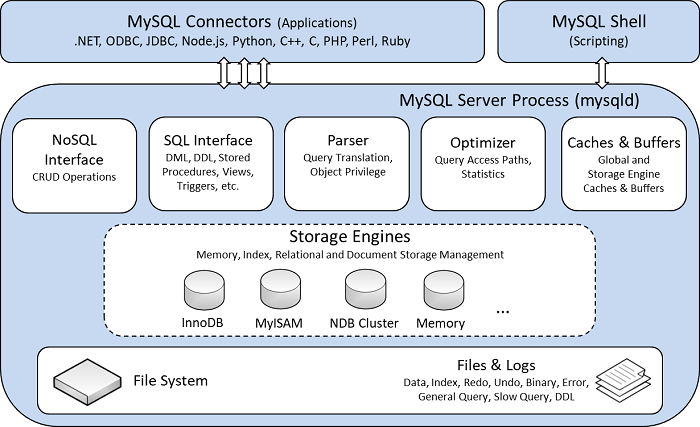
\includegraphics[width=0.8\linewidth]{pics/mysql-architecture.png}
\caption{MySQLのプラガブルストレージエンジンアーキテクチャ（出典：MySQL Reference Manual \\ \url{https://dev.mysql.com/doc/refman/8.0/ja/pluggable-storage-overview.html} ）}
\label{fig:mysql}
\end{figure}

第二に，MySQLとLineairDBを接続するhandlerを実装した。MySQLは，サーバ層とストレージエンジン層が分離された構造を持ち，SQLの実行結果はhandlerインターフェースを通じてストレージエンジンに伝達される（図\ref{fig:mysql}）。そのため，Kamoを実現するには，MySQLから受け取ったテーブル操作やレコード操作をLineairDBのAPIに変換するhandlerが必要であった。本プロジェクトではこのhandlerを実装することで，MySQL互換のSQLインターフェースを維持したまま，内部ではLineairDBによる高速なトランザクション処理を利用できるようにした。

第三に，耐障害性と可用性を付与するための構成を実装した。当初はRaftの導入も検討したが，MySQL本体への大規模な改変が必要であり，開発期間内での実現可能性を踏まえて方針を変更した。最終的には，MySQL標準のSemi-Synchronous Replicationを採用し，さらにOrchestratorによるPrimary障害の自動検知とReplicaの昇格，ProxySQLによる接続先制御を組み合わせることで，自動Failoverを実現した。これにより，障害発生時にもサービスを継続可能な構成を整備した。

以上の開発により，KamoはMySQL互換のインターフェースを維持したまま，業界標準のOLTPベンチマークであるTPC-Cワークロードを実行可能なシステムとなった。TPC-Cを実行できることは，単に基本的なSQL処理が可能であることにとどまらず，複数テーブル，更新処理，索引アクセスを含む実用的なトランザクション処理を支えられることを示すうえで重要である。しかしながら、機能が備わっていても性能が高くなければ意味がない。そのため、開発したKamoについて，TPC-Cワークロードを用いて既存のMySQL と性能比較を行った。

実験環境は表\ref{tab:setup}に，また可用性を付与するための構成は表\ref{tab:proxysql_setup}に示す。これらの構成のもとで評価を行った結果を図\ref{fig:proxysql_tpcc}に示す。結果から，Kamoは分散環境下において既存のMySQLに対して最大18.7倍の性能を示すことがわかった。

\begin{table}[htbp]
\centering
\caption{実験環境}
\label{tab:setup}
\begin{sftabular}{p{4cm}p{10cm}}
\hline
項目&内容\\
\hline
構成&DBノード3台（Primary1台+Replica2台，同一スペック）\\
CPU&AMDEPYC9654P96-CoreProcessor（192vCPU）\\
メモリ&1.0TiB\\
ストレージ&1TB（実効容量993GB）\\
OS&Ubuntu22.04.5LTS\\
カーネル&Linux5.15.0-119-generic\\
仮想化基盤&KVM（仮想マシン）\\
レプリケーション方式&MySQL Semi-Synchronous Replication\\
\hline
\end{sftabular}
\end{table}

\begin{table}[h]
\centering
\caption{ProxySQLノードの構成}
\begin{sftabular}{ll}
\hline
項目&仕様\\
\hline
CPU&IntelXeonGold6212U@2.40GHz（20vCPU）\\
メモリ&31GiB\\
ストレージ&約500GB（実効容量約405GB）\\
OS&Ubuntu22.04.5LTS\\
カーネル&Linux5.15.0-121-generic\\
\hline
\end{sftabular}
\label{tab:proxysql_setup}
\end{table}

\begin{figure}[htbp]
\centering
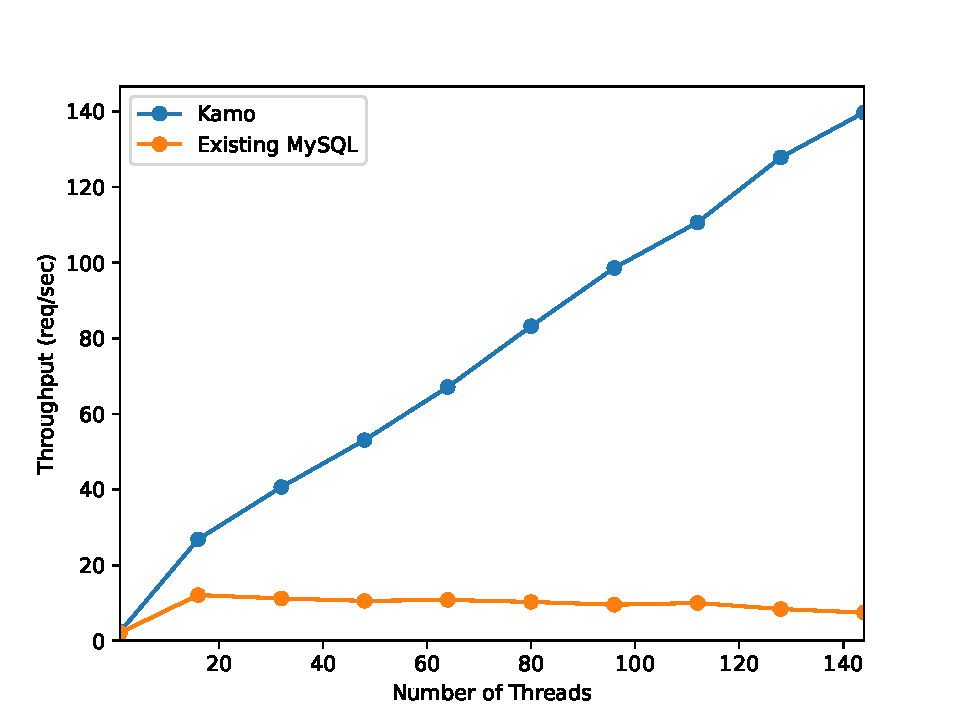
\includegraphics[width=0.8\linewidth]{pics/proxysql_tpcc.pdf}
\caption{ProxySQL構成におけるTPC-CワークロードでのKamoと既存のMySQLの比較}
\label{fig:proxysql_tpcc}
\end{figure}

\section{従来の技術との相違}

従来のMySQLは，成熟した互換性と豊富な利用実績を持つ一方で，マルチコア環境におけるスケーラビリティには改善の余地がある。本プロジェクトは，そのMySQLを置き換えるのではなく，プラガブルストレージエンジン機構を活用することで，MySQL互換のまま高性能化を図った点に特徴がある。

また，単にLineairDBを接続しただけではなく，RDBMSに必要な\texttt{Table}，\texttt{Insert}/\texttt{Update}/\texttt{Delete}，\texttt{Secondary Index}，走査機構などを新たに実装し，MySQLのhandlerと接続することで，SQLから透過的に利用できるようにした。すなわち，本プロジェクトの新規性は，高性能なKey-ValueストアをMySQL互換DBMSのストレージエンジンとして成立させるために必要な機能群を実装した点にある。

さらに，耐障害性についても，既存のMySQLレプリケーション機構にProxySQLとOrchestratorを組み合わせることで，自動Failoverを含む実運用可能な構成を実現した。これは単なるベンチマーク用試作にとどまらず，高性能性と可用性の両立を目指した実践的なシステム開発である。
\section{期待される効果}

本プロジェクトの成果は，MySQL互換のSQLインターフェースを維持したまま，高性能化と耐障害性の向上を両立できる点に意義がある。MySQLは広く利用されている主要なDBMSであり，その互換性を保ったまま性能向上が可能になれば，既存アプリケーション資産を活かしつつ導入できるため，Webサービス，E-commerce，金融系システム，企業情報システムなど，MySQLを利用する幅広い分野への波及が期待される。

技術的効果としては，既存のMySQLでは十分に活かしきれなかったマルチコア環境での高並列処理性能を，引き出せる可能性がある。実際に，本プロジェクトで開発したKamoは，192 vCPU・3 台構成の評価環境において，TPC-Cワークロードで既存のMySQLに対して最大18.7倍の性能を示しており，高負荷なOLTP処理を扱うシステムにおいて，処理能力の向上やサーバ資源の有効活用に寄与することが期待される。

また，可用性の面では，MySQL標準のSemi-Synchronous Replicationに加え，ProxySQLおよびorchestratorを組み合わせることで，障害検知，接続先切替，Primary昇格までを含む自動Failover構成を実現している。これにより，障害時にもサービス継続が求められる実運用環境への適用可能性を高める効果がある。

さらに，本プロジェクトは，高性能なKey-ValueストアをMySQL互換DBMSのストレージエンジンとして成立させるための技術蓄積という点でも意義がある。今後の高性能DBMS，MySQL拡張技術，高可用データベース基盤の研究開発を活性化することが期待される。

\section{普及の見通し}

本プロジェクトで開発したKamoは，MySQL互換のSQLインターフェースを維持しつつ，高性能化と耐障害性の向上を目指したDBMSである。そのため，既存のMySQLを利用している開発者や運用者にとって，比較的導入を検討しやすい構成になっている。特に，高負荷なOLTP処理を扱うWebサービス，E-commerce，業務システムなどにおいて，既存アプリケーション資産を活かしたまま性能改善を図る手段として普及することが期待される。

また，本プロジェクトで得られた成果は，単なる試作にとどまらず，高性能なKey-ValueストアをMySQL互換DBMSのストレージエンジンとして成立させるための実装知見を含んでいる。そのため，データベースシステムや高性能トランザクション処理の研究分野においても，今後の研究開発の基盤として活用される可能性がある。特に，MySQLの互換性を保ちながら内部実装を刷新するという方向性は，既存DBMSの性能改善や高可用化を検討する上で有用な事例になると考えられる。

今後は，OSSとしての公開に向けて，導入方法や制約事項を含むドキュメント整備を進めるとともに，性能評価結果や運用手順を整理し，利用しやすい形で提供していく予定である。さらに，学会や技術コミュニティでの発表を通じて認知を広げることで，研究用途に加えて，実サービス基盤への適用可能性も高めていきたい。将来的には，性能と可用性の両立が求められるシステムにおいて，本成果を発展させた技術が広く利用されることを目指している。

\section{クリエータ名（所属）}
\begin{itemize}
  \item 宮﨑 祐介（慶應義塾大学 総合政策学部 総合政策学科）
  \item 中森 辰洋（慶應義塾大学 大学院政策・メディア研究科）
  \item 李 浩文（慶應義塾大学 大学院政策・メディア研究科）
\end{itemize}

\section*{（参考）関連URL} % もしあれば
% 関連URLは参考文献のリンクではなくプロジェクト・プロダクトに直接関係するものへのリンクです。成果詳細では参考文献を貼るのはなしです。
\begin{itemize}
  \item ソースコード：\url{https://github.com/mitou-Kamo/LineairDB-storage-engine}
\end{itemize}

\end{document}
